\documentclass[12pt]{article}
\usepackage{amsmath,amssymb}
\usepackage{color}
\usepackage{enumitem}
\usepackage{hyperref}
\usepackage{listings}
\usepackage{graphicx}

\lstset{
  basicstyle=\ttfamily,
  mathescape
}

% MAKE TITLE AND AUTHOR
\title{Natural language processing}
\author{
    Andrea Auletta
    \and
    Aulo
}

\date{\today}
\makeindex
\begin{document}
\maketitle
\tableofcontents
\newpage


\section{Text summarization with pretrained encoders}
\subsection{Some definitions}
\begin{itemize}
    \item \textbf{Good summary}: A good summary must be fluent and consistent, capture all the important topics, but not contain repetitions 
    of the same information;
    \item \textbf{Abstractive modeling}: the task requires language generation capabilities in order to create 
    summaries containing novel words and phrases not featured in the source text;
    \item \textbf{Extractive summarization}: is often defined as a binary classification task with labels 
    indicating whether a text span (typically a sentence) should be included in the summary;
    \item \textbf{Pretrained language model}: extends the idea of word embeddings by learning representations
    from large-scale corpora using a language modeling objective.
\end{itemize}
\subsection{Summary}
Here they explore the potential of Bert under a general framework encompassing both extractive 
and abstractive summarization. They combine the Pretrained Bert with a randomly-initialized Transformer 
decoder. The difference here is that we eant to manipulate multi-sentential input w.r.t. the usual task of Bert.
In Bert for summarization the document representations are learned hierarchically where lower transformer layers
represent adjacent sentences, while higher layers (+self-attention) represent multi-sentence discourse.
\begin{center}
    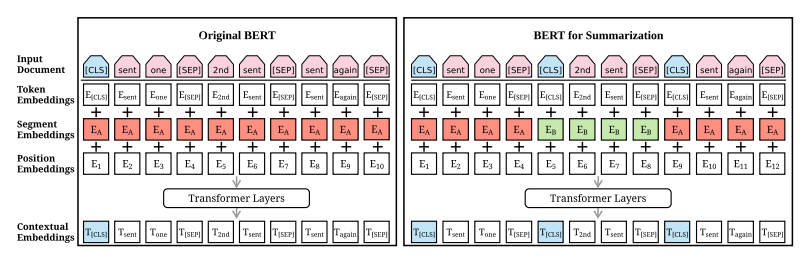
\includegraphics[scale=0.6]{./img/bert.png}
\end{center}
\subsubsection{Extractive summarization}
With BertSum we have the vector $v_i$ of the i-th [CLS] symbol from the top layer can be used as the 
representation of the i-th sentence. After this we have other inter-sentence transformer layers 
to capture document-level featurs for extracting summaries. The output layer is a sigmoid classifier.
\subsubsection{Abstractive summarization}
Standard encoder-decoder framework is used. The encoder is BertSum and the decoder is a 6-layered Transformer
initialized randomly. 
To circumvent the fact that the decoder is not pretrained is designed a new fine-tuning method: Adam 
optimizer with $\beta_1=0.9$ and $\beta_2=0.999$ for the encoder and the decoder, each with different
warmup-step and learning rates: 
\begin{itemize}
    \item $lr_\epsilon = \tilde{lr}_\epsilon \cdot min(step^{-0.5}, step \cdot warmup_\epsilon^{-1.5})$, 
    where $\tilde{lr}_\epsilon=2e^{-3}$, $warmup_\epsilon=20000$ for the encoder;
    \item $lr_\mathcal{D} = \tilde{lr}_\mathcal{D} \cdot min(step^{-0.5}, step \cdot warmup_\mathcal{D}^{-1.5})$, 
    where $\tilde{lr}_\mathcal{D}=0.1$, $warmup_\mathcal{D}=10000$ for the decoder;
\end{itemize}
The encoder can be trained with more accurate gradients when the decoder is becoming stable.
\subsection{implementation}
\begin{itemize}
    \item PyTorch;
    \item OpenNMT;
    \item bert-based-uncased: https://git.io/fhbJQ; 
    \item dropout for abstractive models;
    \item rouge-2 score for extractive models against gold summary (selct the top 3 sentences);
    \item Summarization quality using Rouge (1, 2, L)
    \item human evaluation.
\end{itemize}
\section{Automatic Text Summarization: a State-of-the-art Review}
\subsection{Extractive methods}
The main task is to determine which sentences are important and should 
be included in the summary. 
\begin{itemize}
    \item Cheng: data-driven approach for single-document summarization based on continuous a 
    hierchical document encoder and an attention-based extractor. The model can be trained on large-scale
    datasets and learn informativeness features based on continuous representations without 
    access to linguistic annotations. The labels are assigned to each sentence in the 
    document individually based on their semantic correspondence with the gold summary;
    \item Nallapati: recurrent neural network based sequence model for extractive single-document
    summarization (SummaRuNNer). Identify the set of sentences which collectively collectively give the 
    highest ROUGE with respect to the gold summary
    \item Narayan: similar approach but for sentence ranking there is a combination of maximum-likelihood cross-entropy
    with rewards from policy gradient reinforcement learning to direclty optimize the final evaluation
    metric (ROUGE), a sentence gets a high rank for summary selection if it often occurs in high
    scoring summaries.
    \item Yasunaga: GCN takes sentence embedding from RNN as input node feature and through 
    multiple layers-wise propagation generates high-level hidden features for sentences. Sentence salience is then estimated
    through a regression on top and the important sentences are extracted in a greedy 
    manner while avoiding redundancy.

\end{itemize}
\end{document}